\section{Environmental Permit Application Process}
\label{sec:environmental-permit-application-process}
In this section, methodology proposed in this thesis study will be applied on the \textit{Environmental Permit Application Process} dataset \cite{coselog-data} and evaluation results will be presented with a similar approach above. Since this dataset consists of real-life event logs, preprocessing is undertaken prior to start analysis. Incomplete traces, which started but not ended in the time frame of log collection, and exceptional cases are removed from event logs with the help of ProM log visualization tools with a similar approach in \cite{buijs2014flexible}. Statistical information about the dataset that is used in this section can be summarized in Table~\ref{table:coselog-process-summary}.

%\caption{Statistical summary of Environmental Permit Application Process dataset}
%\label{table:coselog-process-summary}
 \begin{table}[]
\centering
\caption{Statistical summary of Environmental Permit Application Process dataset}
\label{table:coselog-process-summary}
\begin{tabular}{lccc}
\hline
                       & {\bf Cases} & {\bf Events} & {\bf Percentage} \\ \hline
{\bf Municipality \#1} & 54          & 131          & 6.1 \%           \\ \hline
{\bf Municipality \#2} & 302         & 586          & 27.3 \%          \\ \hline
{\bf Municipality \#3} & 37          & 73           & 3.4 \%           \\ \hline
{\bf Municipality \#4} & 340         & 507          & 23.7 \%          \\ \hline
{\bf Municipality \#5} & 481         & 845          & 39.4 \%          \\
{\bf Total}            & {\bf 1214}  & {\bf 2142}   & {\bf }           \\ \hline
\end{tabular}
\end{table}

As shown in Table~\ref{table:coselog-process-summary}, total of 1214 cases and 2142 events included in this dataset with a variable distribution between event logs of municipalities. In the following sections, these municipalities will be used as organizational logs and the methodology presented in this thesis study will be applied.

\subsection{Methodology Stages}
\label{sec:coselog-methodology}
In \textit{Process Model Mining} stage, event logs of each municipality in the dataset are used as organizational event logs and they are used to mine process models. Considering preprocessing is undertaken on the event logs, noise threshold in \textit{Inductive Miner} is set to a low value of 10\% to achieve a higher fitness. 

Appropriateness and fitness evaluation metrics are summarized in Table~\ref{table:coselog-wabo-process-model-mining} and it can be seen that each event log is successful in terms of representing reality with high fitness values. However, some of the process models like Municipality #5 and #4 resulted with low appropriateness values. Process models for each event log are visualized with a detail simplification based on number of activities and paths in Figure~\ref{fig:coselog-wabo-process-models} and it can be seen that low appropriateness values resulted with complicated process models that are difficult to analyze visually. Detail simplification is only used for visualization and it draws the mainstream process flow instead of whole set of paths and activities. It should be kept in mind that actual process models are 5 to 10 times more complicated than the ones presented in Figure~\ref{fig:coselog-wabo-process-models}.

%\caption{Process Model Mining Evaluation of Environmental Permit Application Process Dataset}
%\label{table:coselog-wabo-process-model-mining}
\begin{table}[]
\centering
\caption{Process Model Mining Evaluation of Environmental Permit Application Process Dataset}
\label{table:coselog-wabo-process-model-mining}
\begin{tabular}{lcccc}
\hline
 & {\bf Fitness} & {\bf \begin{tabular}[c]{@{}c@{}}Structural\\Appropriateness\end{tabular}} & {\bf \begin{tabular}[c]{@{}c@{}}Behavioral\\Appropriateness\end{tabular}} & {\bf \begin{tabular}[c]{@{}c@{}}Average\\Appropriateness\end{tabular}} \\ \hline
{\bf Municipality \#1} & 86 \% & 97.5 \% & 54.4 \% & 76 \% \\ \hline
{\bf Municipality \#2} & 100 \% & 100 \% & 100 \% & 100 \% \\ \hline
{\bf Municipality \#3} & 92.3 \% & 71.1 \% & 67.2 \% & 69.1 \% \\ \hline
{\bf Municipality \#4} & 96.8 \% & 65.7 \% & 64 \% & 64.9 \% \\ \hline
{\bf Municipality \#5} & 94.5 \% & 58.8 \% & 39.7 \% & 49.3 \% \\ \hline
{\bf Average} & {\bf 93.9 \%} & {\bf 78.6 \%} & {\bf 65.1 \%} & {\bf 71.9 \%} \\ \hline
\end{tabular}
\end{table}

\todo{FIGUREx5 ekle!}


In \textit{Performance Indicator Analysis} stage, alignment costs are calculated over replay of event logs on process models. As presented in the Table~\ref{table:coselog-wabo-replay}, as appropriateness and fitness decrease alignment costs increase for the municipalities. This indicates the fact that both process model mining stage and replay stage is in conformity and performance indicators calculated over replay are acceptable.
%\caption{Replay Evaluation of Environmental Permit Application Process Dataset}
%\label{table:coselog-wabo-replay}
\begin{table}[]
\centering
\caption{Replay Evaluation of Environmental Permit Application Process Dataset}
\label{table:coselog-wabo-replay}
\begin{tabular}{lccc}
\hline
 & {\bf Fitness} & {\bf Average Appropriateness} & {\bf Alignment Cost} \\ \hline
{\bf Municipality \#1} & 86 \% & 76 \% & 173.2 \\ \hline
{\bf Municipality \#2} & 100 \% & 100 \% & 0 \\ \hline
{\bf Municipality \#3} & 92,3 \% & 69,1 \% & 332.3 \\ \hline
{\bf Municipality \#4} & 96,8 \% & 64,9 \% & 9,1 \\ \hline
{\bf Municipality \#5} & 94,5 \% & 49,3 \% & 35.8 \\ \hline
\end{tabular}
\end{table}
After calculating the performance indicators, municipalities are clustered based on these values and this stage is evaluated by the within-SSE values for different number of clusters as plotted in Figure~\ref{fig:coselog-wabo-cluster-sse-plot}. In order to avoid overfitting of clusters, number of clusters, \textit{k}, is selected to be 2 for this dataset for further analysis. 
\begin{figure}
	\centering
	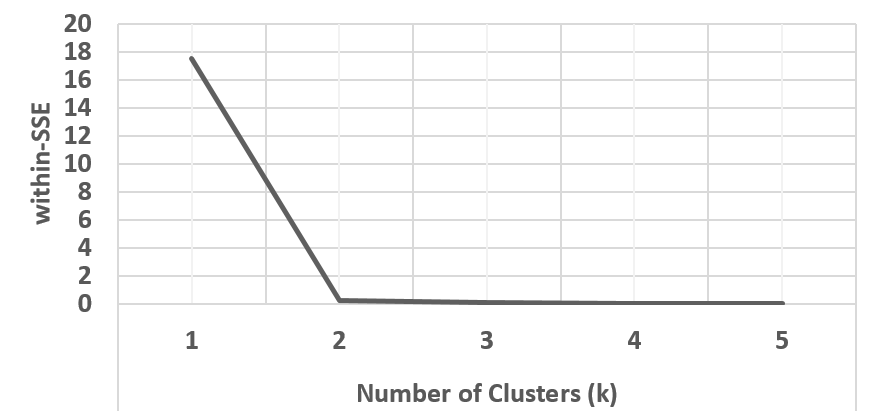
\includegraphics[width=.7\textwidth]{5_results_discussions/coselog-wabo/cluster-sse-plot}
	\caption{Number of Clusters vs. Within-SSE for  Environmental Permit Application Process Dataset}
  \label{fig:loan-cluster-sse-plot}
\end{figure}

In \textit{Mismatch Pattern Analysis} stage,
 % BartHompes paketi ile ikili ikili çalıştır- run


In \textit{Recommendation Generation} stage,
% Responsiveness

\subsection{Discussions}
\label{sec:coselog-discussions}